En esta sección presentamos las herramientas utilizadas para este trabajo.

\subsection{Festival y Festvox}

Festival es un framework que permite sintetizar habla. Además posee una gran variedad de APIs, para el procesamiento de audios y generación de nuevos TTS.

Festvox a su vez expande sobre Festival, agregando todavía mas herramientas relacionadas a la síntesis y generación de modelos, que van desde la generación de modelos prosódicos, hasta etiquetado automático de corpus.

Para este trabajo utilizaremos Festival y festvox para generar los Utternaces requeridos tanto para el entrenamiento como para la síntesis de audios. Estos consisten básicamente en una transcripción fonética de los audios dividida en segmentos temporales y datos contextuales tales como la cantidad de silabas en la palabra siendo transcrita, fonemas que preceden y proceden al actual, etc.

En particular, Festival también cuenta con herramientas de etiquetado automático. Para este trabajo utilizaremos EHMM alingnment, que a partir de un corpus y sus transcripciones, permite generar utternaces cuyos segmentos coinciden con aquellos de los audios.

Como veremos mas adelante, estos utternaces serán utilizados en el entrenamiento con HTS para modelar cada uno de los fonemas.

\subsection{HTS}

HTS es un framework de entrenamiento y sintesis de sistemas TTS basado en HMMs que modela simultáneamente la duración, el espectro (mel-cepstrum) y la frecuencia principal ($f0$) de utilizando una combinación de HMMs:

\begin{figure}
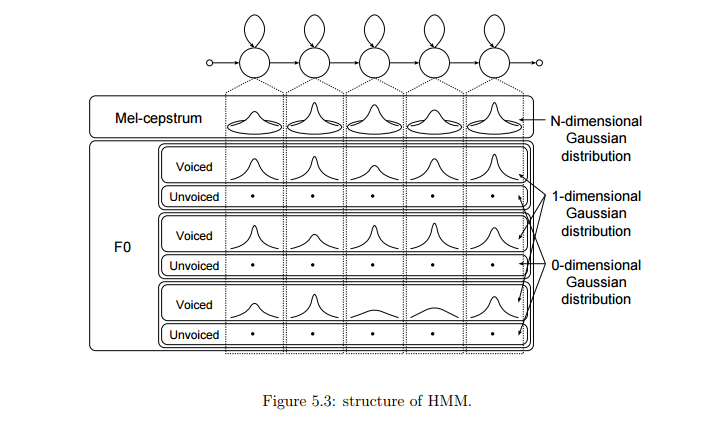
\includegraphics[scale=0.5]{imagenes/hmm.png}
\caption{Estructura de un hmm (simultaneous modeling of phonetic and prosodic parameters, and characteristic conversion for hmm-based text-to-speech systems, takayoshi yoshimura, january 2002, pag. 41)}
\centering
\end{figure}

Mel-celpstum (espectro) y los tres vectores del $f0$ (frecuencia principal) son modelados en paralelo. 

\explicar

Por otro lado HTS toma la decisión de modelar la información prosódica dentro de este mismo framework. Para esto, las distribuciones para el espectro, la frecuencia principal y las duraciones son clusterizadas independientemente utilizando la información contextual extraída de los audios de entrenamiento. A continuación se presenta una vista esquemática de la estructura del HMM generado clusterizado con arboles de decisión:

\begin{figure}
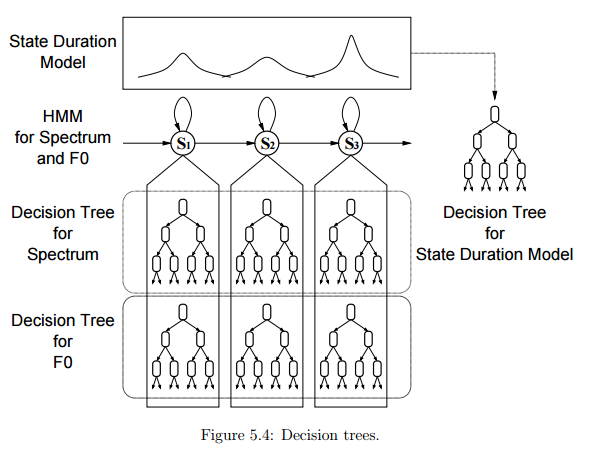
\includegraphics[scale=0.5]{imagenes/hmmContext.png}
\caption{Esquema HMM generado utilizando arboles de decisión (simultaneous modeling of phonetic and prosodic parameters, and characteristic conversion for hmm-based text-to-speech systems, takayoshi yoshimura, january 2002, pag. 45)}
\centering
\end{figure}

%hablar de los distintos tipos de clusters?

En particular para este trabajo la clusterización de datos se realizó generando arboles de decisión y para cada fonema se tomó los dos fonemas precedentes y los dos fonemas procedentes y se extrajo la siguiente información contextual.


\begin{itemize}
\item Modo de articulación del fonema.
\item Punto de articulación del fonema.
\item La perspectiva articulatoria (anterior, central o posterior).
\item Si el fonema es una vocal o una consonante.
\item En caso de ser una vocal, a que categoría pertenece: por ejemplo para el fonema $/i/:$ {$i$ (no acentuada), $i0$ (diptongo) ,$i1$ (acentuada)}.
\item En caso de ser una vocal, su redondeamiento vocálico.
\item En caso de ser una consonante, si es lennis o fortis.
\end{itemize}

En la siguiente imagen se muestra un fragmento de un árbol de decisión generado para modelar la duración de los fonemas en un hmm:

\begin{figure}
\begin{center}
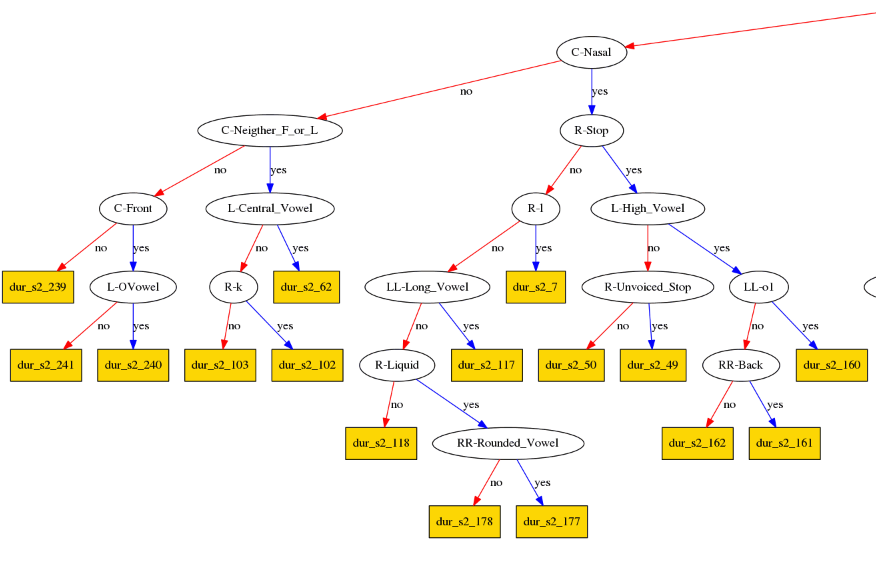
\includegraphics[scale=0.4]{imagenes/arbolDeDesicionTesis.png}
\caption{Árbol de decisión generado para la duración de un HMM}
\end{center}
\end{figure}

Con este modelo, el sistema podrá inferir por ejemplo cosas como: si el fonema actual no es nasal (C-Nasal) seguido de un stop (R-Stop), que no es el fonema $l$ estará modelado por función de probabilidad gaussiana definida en $dur\_s2\_7$.

En las primeras iteraciones del desarrollo no contábamos con la información acústica por lo que se generaron modelos carentes de información contextual. En estos primeros modelos se pudo apreciar una calidad mucho peor en los audios generados, sonando estos sumamente metálicos y carentes de prosodia. Tras agregar los factores contextuales y realizar algunas pruebas de concepto con ellas pudimos comprobar que las voces sonaban mucho mas humanas.

%HTS también brinda la posibilidad de realizar speaker-adaptive training. Esta técnica permite tomar un modelo ya entrenado y adaptarlo para asimilar características de un nuevo hablante. Esta técnica nace de la idea que construir un corpus de datos es costoso tanto en espacio de almacenamiento, tiempo de grabación y etiquetado, por lo que resulta mas económico generar una nueva voz sintética a partir de un modelo bien generado y adaptándolo luego con características del nuevo corpus.

\enganchar
%Dentro del adaptative training existen varias técnicas, en este trabajo utilizaremos offline supervised adaptation, que tiene como requisito adicional conocer los utternaces del segundo corpus. 

% Cosas para hablar:
% contextual factors: cuales son, para que sirven.
% arboles de decición.
% questions
% expandir sobre hmms

\subsection{HTS\_engine}

Finalmente para generar voces con acento extranjero se utilizó hts\_engine. Esta herramienta permite interpolar con pesos arbitrarios entre varios modelos para producir un nuevo modelo con una mezcla de la carga fonética y prosódica de ambos hablantes y sintetizar audios. Esto nos brinda un gran rango exploratorio y nos permitirá ajustar la carga fonética de los modelos originales para acercarnos al modelo deseado. 

